%
% File acl2014.tex
%
% Contact: giovanni.colavizza@epfl.ch
%%
%% Based on the style files for ACL-2013, which were, in turn,
%% Based on the style files for ACL-2012, which were, in turn,
%% based on the style files for ACL-2011, which were, in turn, 
%% based on the style files for ACL-2010, which were, in turn, 
%% based on the style files for ACL-IJCNLP-2009, which were, in turn,
%% based on the style files for EACL-2009 and IJCNLP-2008...

%% Based on the style files for EACL 2006 by 
%%e.agirre@ehu.es or Sergi.Balari@uab.es
%% and that of ACL 08 by Joakim Nivre and Noah Smith

\documentclass[11pt]{article}
\usepackage{acl2014}
\usepackage{times}
\usepackage{url}
\usepackage{latexsym}
\usepackage{graphicx}
\graphicspath{ {./images/} }

%\setlength\titlebox{5cm}

% You can expand the titlebox if you need extra space
% to show all the authors. Please do not make the titlebox
% smaller than 5cm (the original size); we will check this
% in the camera-ready version and ask you to change it back.


\title{Smart recipes}

\author{Omar Mehio \\
  {\tt\small omar.mehio@epfl.ch} \\\And
  Leonardo Perrone \\
  {\tt\small leonardo.perrone@epfl.ch} \\\And
  Attila Bekker \\
  {\tt\small attila.bekker@epfl.ch} \\}

\date{16th of December, 2018}

\begin{document}
\maketitle
\begin{abstract}
  The aim of this document is to find correlations between attributes and characteristics of food recipes and the corresponding ratings and reviews given to that recipe.
  Recipes are gathered from the most popular online recipe websites, extracting common attributes and normalizing them between the different representations. Apart from the attributes explicitly included in the recipe descriptions, new properties are being defined by grouping recipe ingredients into different categories. Furthermore, sentiment analysis is performed on the content of recipe reviews, providing a way to determine the corresponding ratings.
  Performing a range of different analysis techniques provides a set of hints and best practices to help recipe authors to maximize their ratings by choosing the recipes with attributes most likely to be rated positively.
\end{abstract}

\section{Introduction}

This document has been prepared for the \textbf{Applied Data Analytics} course at EPFL in the Fall of 2018.

\section{Data acquisition}

The recipe data is extracted from the \textit{Cooking recipes} database, which is a collection of HTML documents from a wide variety of websites.

\subsection{Data sources}

The analysis is based on data extracted from the most popular websites containing food recipes. The data included recipes from over 50 websites, all featuring their own format and attributes. The initial analysis showed that a few websites containing the highest number of recipes represent a good portion of the total recipes. Since each website requires a custom scraper to be built, and each website displays different attributes of recipes and their ingredients, the aim was to select a small number of websites which still give a good representation of the entire data set.

\vspace{5mm}
\begin{center}
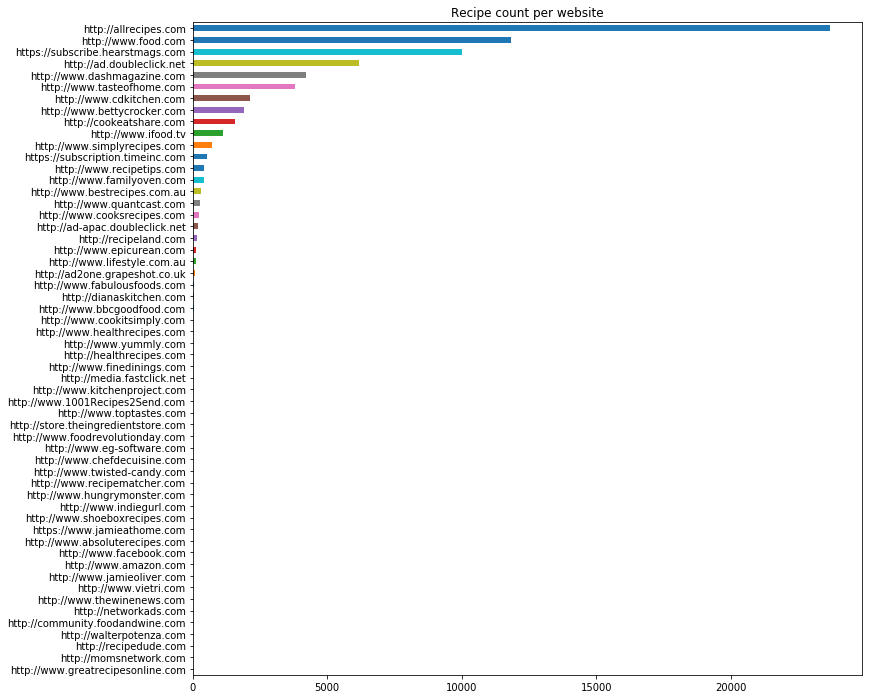
\includegraphics[scale=0.22]{website-count}
\label{website-count} Figure 1. Recipe count
\end{center}
\vspace{5mm}

The top 3 websites containing the most recipes cover about 65\% of all data: 
\begin{enumerate}
\item http://allrecipes.com
\item http://www.food.com
\item https://subscribe.hearstmags.com
\end{enumerate}

\subsection{Data import}

The three selected websites provide different recipe attributes in different formats, which need to be parsed and consolidated into a common format in order to perform meaningful analysis on them.
Common attributes are:
\begin{itemize}
    \item name
    \item review text
    \item review date
    \item rating
    \item category
    \item ingredient list
    \item nutritional values
    \item preparation time
    \item cooking time
    \item difficulty
    \item serving size
\end{itemize}
These attributes may have different scales, different measurement units, or may be missing altogether. 

The three websites require custom scraping algorithms. The source data volume is about 13 GB, which is feasible to be processed on a single computer. The scraping takes 20-30 minutes, the results are stored in \textit{json} format to allow efficient further processing.

\subsection{Data cleaning}

Due to the different formats, the data sets must be cleaned separately. Nutrition information has to be converted to numeric values, using the same measurement units across all recipes. Time values expressed in hours or days need to be converted to minutes. Rating values must be scaled to a common range. Some websites display servings as text, which must be converted to numeric values.

\subsection{Review pre-processing}

The content of the reviews have a special importance for the analysis. In order to analyze the text, a pipeline is constructed to clear the text. Numbers and other non-alphanumeric characters are removed, and all remaining text is converted to lowercase. Stop words offer little value in terms of semantic analysis, so they are being removed. Lemmatizing removes prefixes and suffixes, helping to group similar words. Finally a document term matrix is constructed using both TF-IDF and one-hot encoding matrices.

\section{Preliminary visual analysis}

Once the raw data has been converted into a clean data set with common attributes, they are visualized in order to better understand the characteristics. This analysis is performed before combining the data sets into a single one, allowing comparison between websites.

\subsection{Ratings}

Ratings tend to be dominated by high values. After converting them to a common scale of 3 it can be observed that good ratings highly outnumber bad or medium ones.

\vspace{5mm}
\begin{center}
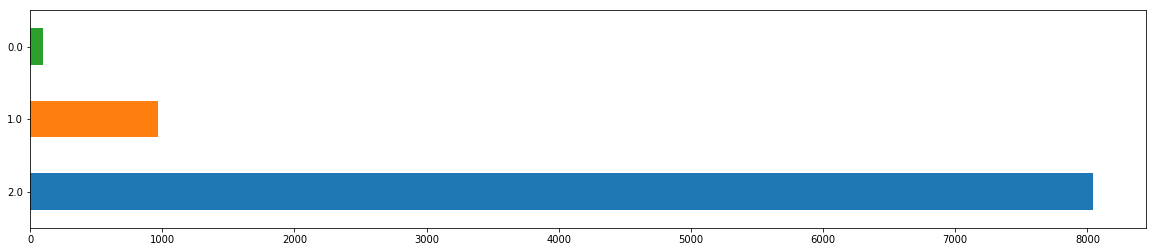
\includegraphics[scale=0.085]{ratings-1}
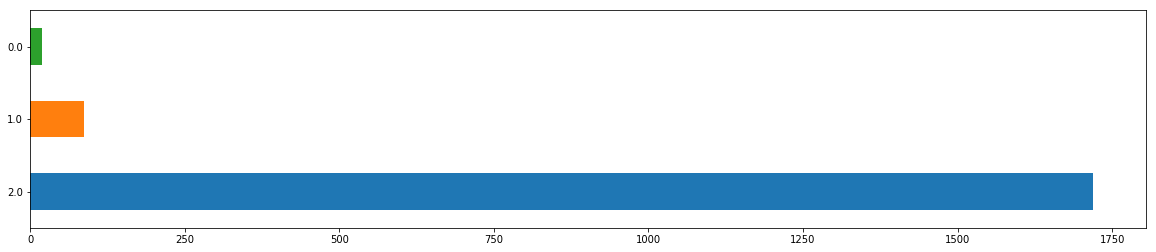
\includegraphics[scale=0.085]{ratings-2}
\label{visalization-ratings} Figure 2. Ratings distribution
\end{center}
\vspace{5mm}

\subsection{Serving size}

Serving sizes range up to 300, but there are only a small number of recipes for more than 50 persons. The 75\% percentile falls to serving sizes of 8 and 12 respectively for the two websites with the most recipes. 

\vspace{5mm}
\begin{center}
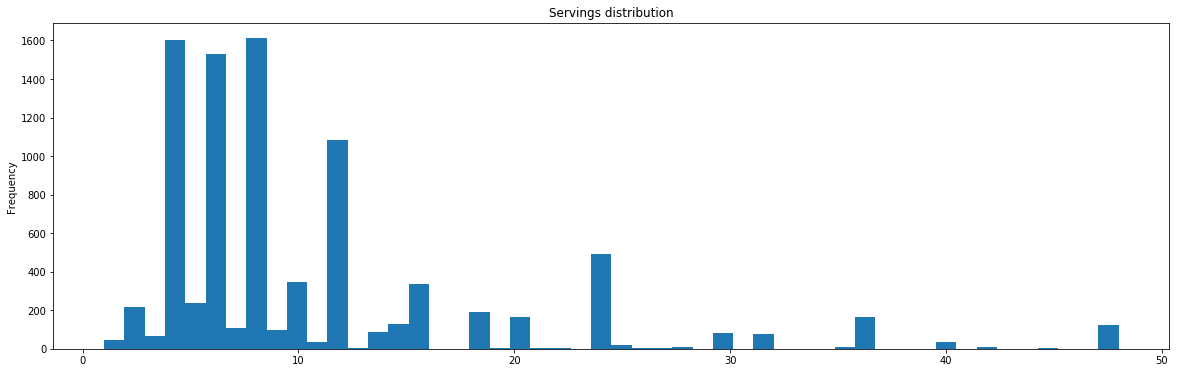
\includegraphics[scale=0.085]{servings-1}
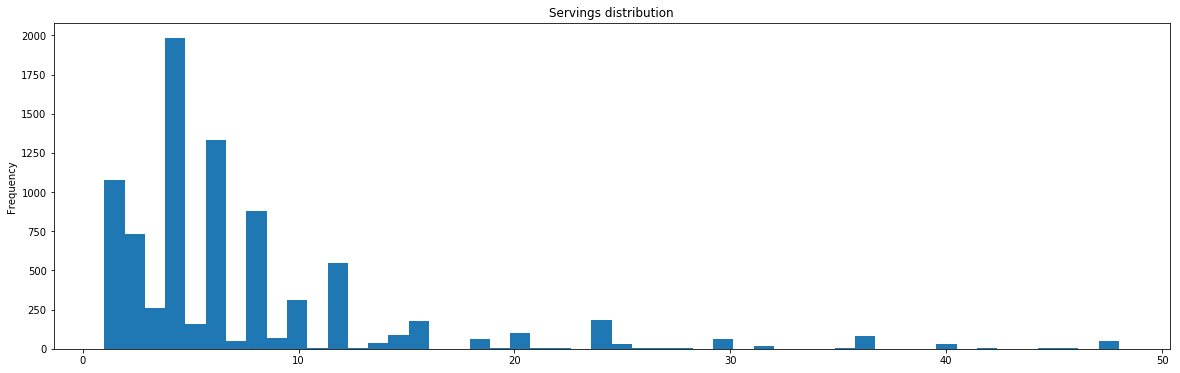
\includegraphics[scale=0.085]{servings-2}
\label{visalization-servings} Figure 3. Servings distribution
\end{center}
\vspace{5mm}

\subsection{Reviews over time}

Most reviews have been created between 2000 and 2010, indicating the period when the data has been collected. The density curves suggest different trends for the popularity of the websites. The allrecipes site shows declining review numbers over the years, while food.com has fairly constant activity, and food-net reviews sharply increase towards the end of the period.

\vspace{5mm}
\begin{center}
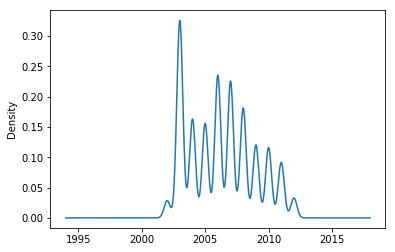
\includegraphics[scale=0.17]{time-1}
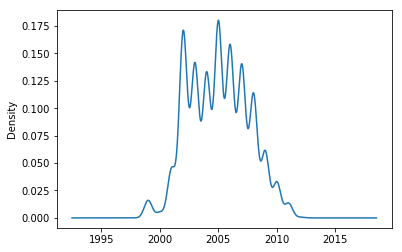
\includegraphics[scale=0.17]{time-2}
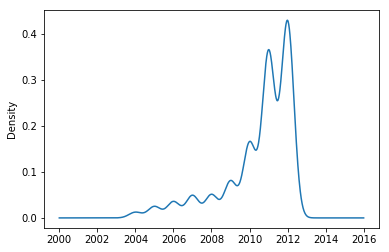
\includegraphics[scale=0.17]{time-3}
\label{visalization-time} Figure 4. Reviews over time
\end{center}
\vspace{5mm}

\subsection{Cooking time}

Cooking times range for a few minutes to several hours, but the distribution shows that most recipes require less than 1 hour cooking, recipes requiring 30 minutes or less being more common.

\vspace{5mm}
\begin{center}
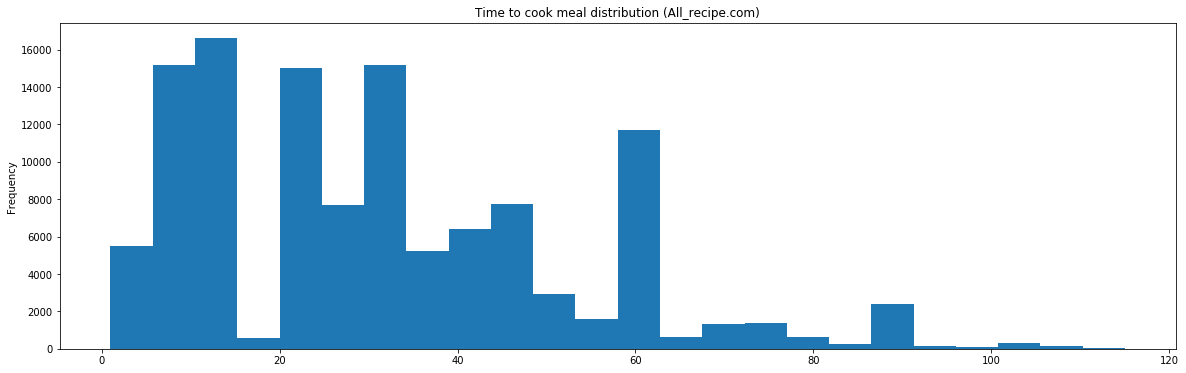
\includegraphics[scale=0.06]{cookingtime-1}
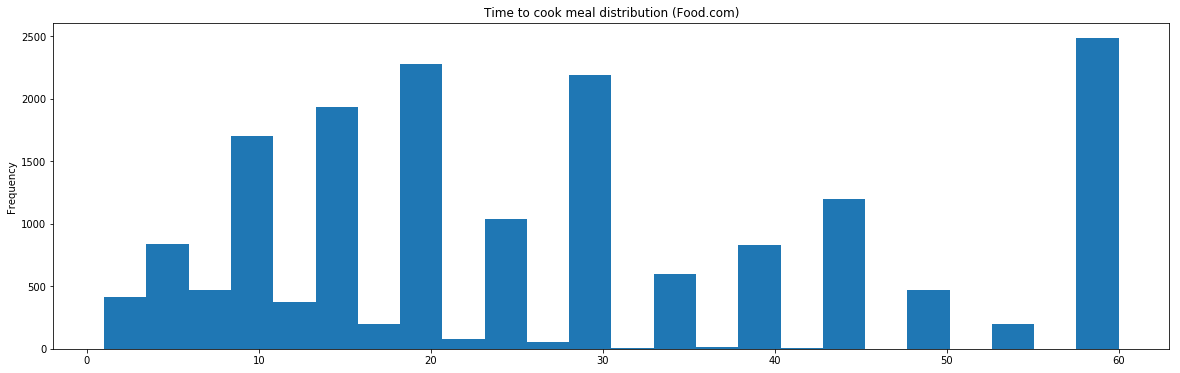
\includegraphics[scale=0.06]{cookingtime-2}
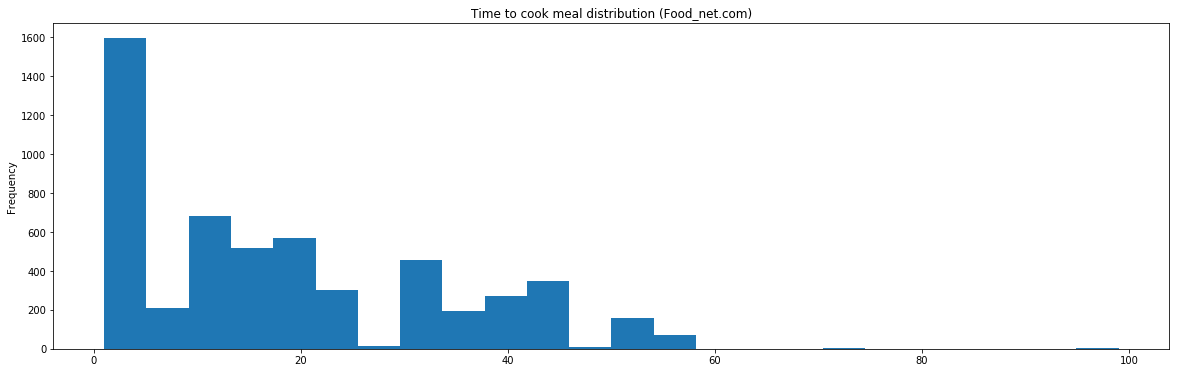
\includegraphics[scale=0.06]{cookingtime-3}
\label{visalization-cookingtime} Figure 5. Cooking time distribution
\end{center}
\vspace{5mm}





\end{document}
